% GNUPLOT: LaTeX picture with Postscript
\begingroup
  \makeatletter
  \providecommand\color[2][]{%
    \GenericError{(gnuplot) \space\space\space\@spaces}{%
      Package color not loaded in conjunction with
      terminal option `colourtext'%
    }{See the gnuplot documentation for explanation.%
    }{Either use 'blacktext' in gnuplot or load the package
      color.sty in LaTeX.}%
    \renewcommand\color[2][]{}%
  }%
  \providecommand\includegraphics[2][]{%
    \GenericError{(gnuplot) \space\space\space\@spaces}{%
      Package graphicx or graphics not loaded%
    }{See the gnuplot documentation for explanation.%
    }{The gnuplot epslatex terminal needs graphicx.sty or graphics.sty.}%
    \renewcommand\includegraphics[2][]{}%
  }%
  \providecommand\rotatebox[2]{#2}%
  \@ifundefined{ifGPcolor}{%
    \newif\ifGPcolor
    \GPcolortrue
  }{}%
  \@ifundefined{ifGPblacktext}{%
    \newif\ifGPblacktext
    \GPblacktexttrue
  }{}%
  % define a \g@addto@macro without @ in the name:
  \let\gplgaddtomacro\g@addto@macro
  % define empty templates for all commands taking text:
  \gdef\gplbacktext{}%
  \gdef\gplfronttext{}%
  \makeatother
  \ifGPblacktext
    % no textcolor at all
    \def\colorrgb#1{}%
    \def\colorgray#1{}%
  \else
    % gray or color?
    \ifGPcolor
      \def\colorrgb#1{\color[rgb]{#1}}%
      \def\colorgray#1{\color[gray]{#1}}%
      \expandafter\def\csname LTw\endcsname{\color{white}}%
      \expandafter\def\csname LTb\endcsname{\color{black}}%
      \expandafter\def\csname LTa\endcsname{\color{black}}%
      \expandafter\def\csname LT0\endcsname{\color[rgb]{1,0,0}}%
      \expandafter\def\csname LT1\endcsname{\color[rgb]{0,1,0}}%
      \expandafter\def\csname LT2\endcsname{\color[rgb]{0,0,1}}%
      \expandafter\def\csname LT3\endcsname{\color[rgb]{1,0,1}}%
      \expandafter\def\csname LT4\endcsname{\color[rgb]{0,1,1}}%
      \expandafter\def\csname LT5\endcsname{\color[rgb]{1,1,0}}%
      \expandafter\def\csname LT6\endcsname{\color[rgb]{0,0,0}}%
      \expandafter\def\csname LT7\endcsname{\color[rgb]{1,0.3,0}}%
      \expandafter\def\csname LT8\endcsname{\color[rgb]{0.5,0.5,0.5}}%
    \else
      % gray
      \def\colorrgb#1{\color{black}}%
      \def\colorgray#1{\color[gray]{#1}}%
      \expandafter\def\csname LTw\endcsname{\color{white}}%
      \expandafter\def\csname LTb\endcsname{\color{black}}%
      \expandafter\def\csname LTa\endcsname{\color{black}}%
      \expandafter\def\csname LT0\endcsname{\color{black}}%
      \expandafter\def\csname LT1\endcsname{\color{black}}%
      \expandafter\def\csname LT2\endcsname{\color{black}}%
      \expandafter\def\csname LT3\endcsname{\color{black}}%
      \expandafter\def\csname LT4\endcsname{\color{black}}%
      \expandafter\def\csname LT5\endcsname{\color{black}}%
      \expandafter\def\csname LT6\endcsname{\color{black}}%
      \expandafter\def\csname LT7\endcsname{\color{black}}%
      \expandafter\def\csname LT8\endcsname{\color{black}}%
    \fi
  \fi
    \setlength{\unitlength}{0.0500bp}%
    \ifx\gptboxheight\undefined%
      \newlength{\gptboxheight}%
      \newlength{\gptboxwidth}%
      \newsavebox{\gptboxtext}%
    \fi%
    \setlength{\fboxrule}{0.5pt}%
    \setlength{\fboxsep}{1pt}%
\begin{picture}(14400.00,5040.00)%
    \gplgaddtomacro\gplbacktext{%
      \csname LTb\endcsname%%
      \put(444,440){\makebox(0,0)[r]{\strut{}\np{e-6}}}%
      \put(444,1097){\makebox(0,0)[r]{\strut{}\np{e-4}}}%
      \put(444,1754){\makebox(0,0)[r]{\strut{}\np{e-2}}}%
      \put(444,2411){\makebox(0,0)[r]{\strut{}\np{1}}}%
      \put(444,3068){\makebox(0,0)[r]{\strut{}\np{e2}}}%
      \put(444,3725){\makebox(0,0)[r]{\strut{}\np{e4}}}%
      \put(444,4382){\makebox(0,0)[r]{\strut{}\np{e6}}}%
      \put(444,5039){\makebox(0,0)[r]{\strut{}\np{e8}}}%
      \put(2588,220){\makebox(0,0){\strut{}$0.05$}}%
      \put(5466,220){\makebox(0,0){\strut{}$0.5$}}%
      \put(576,220){\makebox(0,0){\strut{}$0.01$}}%
      \put(3454,220){\makebox(0,0){\strut{}$0.1$}}%
      \put(6333,220){\makebox(0,0){\strut{}$1$}}%
    }%
    \gplgaddtomacro\gplfronttext{%
      \csname LTb\endcsname%%
      \put(-304,2739){\rotatebox{-270}{\makebox(0,0){\strut{}$\mathcal{K}$}}}%
      \put(3887,-110){\makebox(0,0){\strut{}Mass (GeV)}}%
      \csname LTb\endcsname%%
      \put(1167,4844){\makebox(0,0)[l]{\strut{}$\tau\to\pi$}}%
      \csname LTb\endcsname%%
      \put(1167,4580){\makebox(0,0)[l]{\strut{}$D_s\to e$}}%
      \csname LTb\endcsname%%
      \put(1167,4316){\makebox(0,0)[l]{\strut{}$D_s\to\mu$}}%
      \csname LTb\endcsname%%
      \put(1167,4052){\makebox(0,0)[l]{\strut{}$D_s\to\tau$}}%
      \csname LTb\endcsname%%
      \put(2286,4844){\makebox(0,0)[l]{\strut{}$K\to e$}}%
      \csname LTb\endcsname%%
      \put(2286,4580){\makebox(0,0)[l]{\strut{}$K\to\mu$}}%
      \csname LTb\endcsname%%
      \put(2286,4316){\makebox(0,0)[l]{\strut{}$\pi\to\mu$}}%
      \csname LTb\endcsname%%
      \put(2286,4052){\makebox(0,0)[l]{\strut{}$\pi\to e$}}%
    }%
    \gplgaddtomacro\gplbacktext{%
      \csname LTb\endcsname%%
      \put(7694,440){\makebox(0,0)[r]{\strut{}\np{e-8}}}%
      \put(7694,1590){\makebox(0,0)[r]{\strut{}\np{e-6}}}%
      \put(7694,2740){\makebox(0,0)[r]{\strut{}\np{e-4}}}%
      \put(7694,3889){\makebox(0,0)[r]{\strut{}\np{e-2}}}%
      \put(7694,5039){\makebox(0,0)[r]{\strut{}\np{1}}}%
      \put(9788,220){\makebox(0,0){\strut{}$0.05$}}%
      \put(12666,220){\makebox(0,0){\strut{}$0.5$}}%
      \put(14399,220){\makebox(0,0){\strut{}$2$}}%
      \put(7776,220){\makebox(0,0){\strut{}$0.01$}}%
      \put(10654,220){\makebox(0,0){\strut{}$0.1$}}%
      \put(13533,220){\makebox(0,0){\strut{}$1$}}%
    }%
    \gplgaddtomacro\gplfronttext{%
      \csname LTb\endcsname%%
      \put(11087,-110){\makebox(0,0){\strut{}Mass (GeV)}}%
      \csname LTb\endcsname%%
      \put(8367,1163){\makebox(0,0)[l]{\strut{}$\tau \to \pi$}}%
      \csname LTb\endcsname%%
      \put(8367,899){\makebox(0,0)[l]{\strut{}$\tau\to\mu$}}%
      \csname LTb\endcsname%%
      \put(8367,635){\makebox(0,0)[l]{\strut{}$\tau\to e$}}%
      \csname LTb\endcsname%%
      \put(9486,1163){\makebox(0,0)[l]{\strut{}$K\to\pi e$}}%
      \csname LTb\endcsname%%
      \put(9486,899){\makebox(0,0)[l]{\strut{}$K\to\pi\mu$}}%
      \csname LTb\endcsname%%
      \put(9486,635){\makebox(0,0)[l]{\strut{}$\mu\to e$}}%
    }%
    \gplbacktext
    \put(0,0){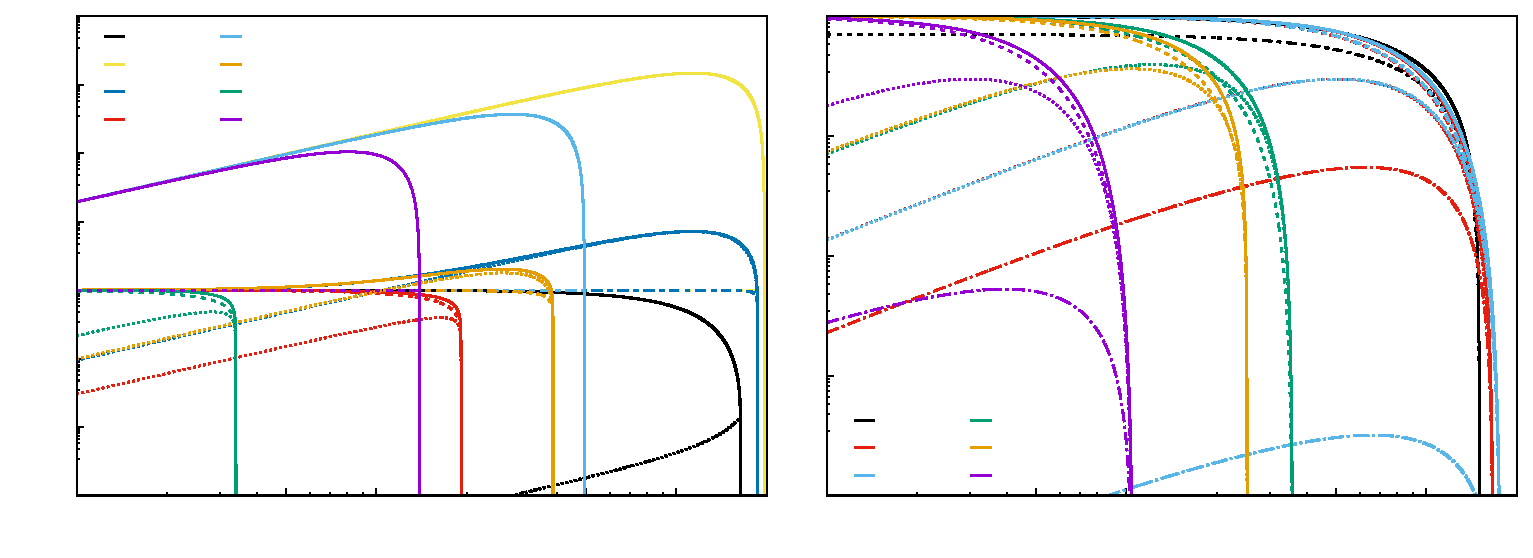
\includegraphics{pics/multiScale_2}}%
    \gplfronttext
  \end{picture}%
\endgroup
